% Chapter 5

\chapter{Project Development Methodology/Architecture}
\label{Chapter5}



This chapter describes the project development methodology and architecture for the RISC-V platform-level interrupt controller (PLIC), which prioritizes and distributes global interrupts in a RISC-V system.\\ 

The PLIC connects global interrupt sources to interrupt targets. The PLIC can be distributed into three modules that are named as PLIC gateway, PLIC register map and PLIC target as explained in the block diagram in figure \ref{fig:block_diagram}. \\

\subsection{PLIC GATEWAY}
The figure \ref{fig:plic_gateway} shows the block diagram of module of the PLIC gateway.\\

\begin{figure}[h]
  \centering
  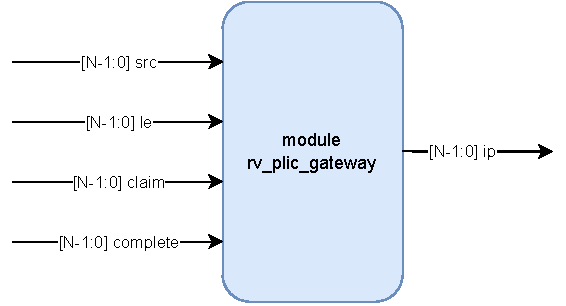
\includegraphics[width=0.95\textwidth]{./fatima_figures/un.drawio.pdf}
  \caption{PLIC Gateway Module.}
  \label{fig:plic_gateway}
\end{figure}

The interrupt gateways in the platform level interrupt controller are responsible for converting global interrupt signals into a common interrupt request format, and for controlling the flow of interrupt requests to the PLIC core. At most one interrupt request per interrupt source can be pending in the PLIC core at any time and it can be indicated by setting the source’s interrupt pending bit. After receiving notification that the interrupt handler servicing the previous interrupt request from the same source has completed, the gateway forwards a new interrupt request to the PLIC core. If the global interrupt source uses level-sensitive interrupts, the gateway will convert the first assertion of the interrupt level into an interrupt request, but thereafter the gateway will not forward an additional interrupt request until it receives an interrupt completion message. If the interrupt is level-triggered and the interrupt is still asserted, a new interrupt request will be forwarded to the PLIC core on receiving an interrupt completion message. The gateway does not have the facility to retract an interrupt request once forwarded to the PLIC core. If a level-sensitive interrupt source de-asserts the interrupt after the PLIC core accepts the request and before the interrupt is serviced, the interrupt request remains present in the IP bit of the PLIC core and will be serviced by a handler, which will then have to determine that the interrupt device no longer requires service. If the global interrupt source was edge-triggered, the gateway will convert the first matching signal edge into an interrupt request. Depending on the design of the device and the interrupt handler, in between sending an interrupt request and receiving notice of its handler’s completion, the gateway might either ignore additional matching edges or increment a counter of pending interrupts. In either case, the next interrupt request will not be forwarded to the PLIC core until the previous completion message has been received. If the gateway has a pending interrupt counter, the counter will be decremented when the interrupt request is accepted by the PLIC.\\

\subsection{PLIC TARGET}
The figure \ref{fig:plic_target} shows the block diagram of module of the PLIC Target.\\

\begin{figure}[h]
  \centering
  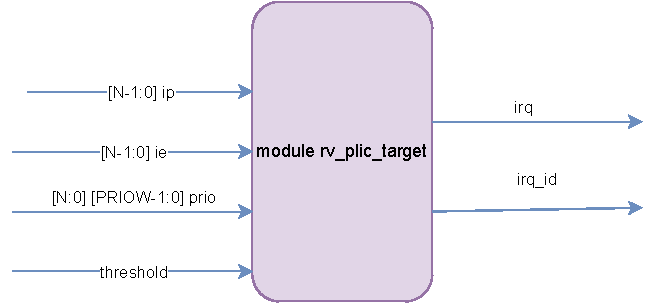
\includegraphics[width=0.95\textwidth]{./fatima_figures/target.drawio.pdf}
  \caption{PLIC Target Module.}
  \label{fig:plic_target}
\end{figure}

The PLIC target deal with the interrupt pending bit, interrupt enable bit, interrupt priority and threshold.\\

The current status of the interrupts pending in the PLIC core can be read from the interrupt pending register. \\

Each target has a vector of interrupt enable (IE) bits, one per interrupt source. The target will not receive interrupts from sources that are disabled. Each global interrupt can be enabled by setting the corresponding bit in the enables register. The IE bits for a single target should be packed together as a bit vector in platform-specific memory-mapped control registers to support rapid context switching of the IE bits for a target. IE bits are WARL fields that can be hardwired to either 0 or 1. Bit 0 of enable register 0 represents the non-existent interrupt ID 0 and is hardwired to 0. \\

The PLIC supports interrupt priorities, that is each PLIC interrupt source can be assigned a priority by writing to its memory-mapped source priority register. A priority value of 0 is reserved to mean never interrupt and effectively disables the interrupt. Priority 1 is the lowest active priority while the maximum level of priority is defined by the max priority parameter. Ties between global interrupts of the same priority are broken by the Interrupt ID; interrupts with the lowest ID have the highest effective priority.\\

The threshold priority level is set via the Priority Threshold Register. An interrupt line with a priority less than the threshold, is masked. As an example, a threshold value of zero permits all interrupts with non-zero priority.\\

\subsection{PLIC Register Map}
The figure \ref{fig:plic_RegMap} shows the block diagram of module of the PLIC Target.\\

\begin{figure}[h!]
  \centering
  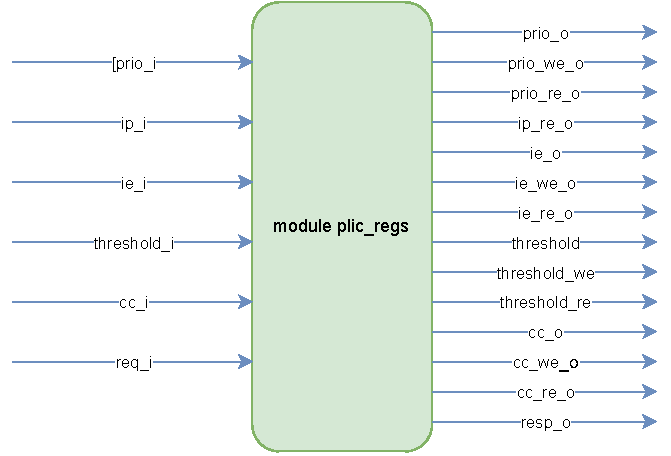
\includegraphics[width=0.95\textwidth]{./fatima_figures/regmap.drawio.pdf}
  \caption{PLIC Target Module.}
  \label{fig:plic_RegMap}
\end{figure}

The register map for the PLIC control registers is shown in table \ref{table:regmap}

\begin{table}[h!]
\centering
 \begin{tabular}{||p{3cm} p{1.5cm} p{1.5cm} p{1.5cm} p{5cm}||} 
 \hline
 \rowcolor{gray}
 Register-Name & Offset(hex) & Size(Bits) & Reset(hex) & Description  \\ [0.5ex] 
 \hline\hline
 \rowcolor{lightgray}
 source priority-0 & 0X0 & 24 & 0X0 & Register holds the priority value of the respective interrupt source\\ 
 \rowcolor{gray}
 source priority-1 & 0X4 & 24 & 0X0 & \\ 
 \rowcolor{lightgray}
 ... & ... & ... & ... & \\
 \rowcolor{gray}
 source priority-31 & 0X7C & 24 & 0X0 & \\ 
 \rowcolor{lightgray}
 source pending & 0X1000 & 32 & 0X0 & Register holds the pending interrupt bits for upto 32 sources in a single register\\
 \rowcolor{gray}
 target enables & 0X2000 & 32 & 0X0 & Register holds the interrupt enable bits for upto 32 sources in a single register\\
 \rowcolor{lightgray}
 target threshold & 0X200000 & 32 & 0X0 & Register holds the priority threshold of the respective target\\
 \rowcolor{gray}
 target claim & 0X200004 & 32 & 0X0 & Register holds interrupt claim/completion information for the respective target\\ [1ex] 
 \hline
 \end{tabular}
 \caption{PLIC Register Map for all configuration registers}
 \label{table:regmap}
\end{table}

Distribute the project goals into smaller objectives/modules and outline deliverables for each objective. Explain the modules of the project through a system-level block diagram. Students may also mention tools, technologies, and suitability of the method(s) to be employed with justification. In case of a research problem, outline the approaches that will be investigated in the project. ($2-3$ pages)

